\chapter{System Design}
Once the requirements of the system had been defined, and a development methodology chosen, the design process could begin. As a phased development methodology was chosen, with two phases, the design process was split into two sections.

\section{Phase One: Generic Optimisation Library}
The first phase of development was the generic optimisation library. As defined by the system requirements, this had to be capable of maximising or minimising any unconstrained real value problem and had to implement the genetic, evolution strategies and particle swarm optimisation algorithms with a number of selection and recombination modes.
\\The first step in designing the library was to select which selection and recombination modes should be implemented. 
\\For the GA, the following selection and recombination methods were chosen
\begin{itemize}
  \item{Proportional selection}
  \item{Rank selection}
  \item{Binary tournament selection}
  \item{One point crossover}
  \item{Two point crossover}
\end{itemize}
These three selection methods were chosen because of their simplicity yet effectiveness. Originally, the GA was implemented with only rank and proportional selection. Binary tournament selection was added later after some initial testing. Only binary tournament support was added, instead of a variable size tournament, in order to avoid adding another configurable parameter which could affect the performance of the GA.
\\ES was implemented with all the selection and recombination methods discussed, so
\begin{itemize}
  \item{$(\mu,\lambda)$ selection}
  \item{$(\mu+\lambda)$ selection}
  \item{Discrete recombination}
  \item{Global discrete recombination}
  \item{Intermediate recombination}
  \item{Global intermediate recombination}
\end{itemize}
The ES algorithm was also implemented using the repair methodology to provide constraint handling. As the requirements of the project specify that the system must be able to deal with any unconstrained problem but must also only optimise within the problem's bounds, constraint handling is used to prevent the ES algorithm from exploring outside the bounds. The repair method used is defined as follows
\begin{algorithm}[h]
\label{alg:esrepair}
  \SetAlgoLined
  \While{value $x_{i}$ violates bound $b_{i}$} {
    $x_{i} -= 1.1 * (x_{i} - b_{i})$;
  } 
  \caption{ES repair algorithm}
\end{algorithm}
\\It was also necessary to choose what type of PSO algorithm to implement; \emph{gbest} or \emph{lbest}. A \emph{gbest} PSO was chosen, for simplicity.  As with ES, the PSO algorithm also needed to be defined with a bound handling algorithm. The bound handling algorithm implemented is a modified version of velocity reflection, where the particle's position is reflected back into the search space by the amount it violated the bound (see algorithm \ref{alg:psoreflect}, adapted from \cite{reflect})
\begin{algorithm}[h]
\label{alg:psoreflect}
  \SetAlgoLined
  \While{value $x_{i}$ violates bound $b_{i}$} {
    \eIf{$b_{i}$ is $x_{max}$}{
      $x_{i} = b_{i} - |x_{i} - b_{i}|$;
    }
    { 
      $x_{i} = b_{i} + |x_{i} - b_{i}|$;
    }
  } 
  \caption{PSO bound handling algorithm}
\end{algorithm}
\\\\Once the specifics of the algorithms had been chosen, the structure of the library could be designed. From the research stage of the project, the general structure and flow of the algorithms were known (see fig. \ref{fig:EA} and algorithm \ref{alg:gbest}). This allowed the focus of the design process to be on the class structure of the system as opposed to the data flow or structure of the algorithms.

\subsection{Class Structure}
The full class diagram for the optimisation library can be seen in appendix \ref{sec:appendix1}; many constructors and public/protected variables have been left out for compactness. The core of this design are the Population, Individual and Chromosome classes.
\\A Population consists of one or more Individuals, stored in a array defined with protected visibility. An array was chosen over one of the generic container classes, such as ArrayList, because the population size is always constant throughout and the system only requires read and write access, so the advantages of using a container class would not be exploited. The array was defined as protected in order to allow subclasses to access it simply and quickly. In order to meet various requirements of the system, the Population class provides functionality to save to and load from a file and store the results of optimisation and plot them on a scatter graph (using JFreeChart\cite{jfree}). 
\\An Individual contains one or more Chromosomes, stored in an array. Again, an array was chosen because the number of chromosomes is constant and only simple access is required. The class implements the Comparable interface because the population of individuals needs to be sortable; individuals are sorted by their normalised fitness value. The Individual class provides methods which allow an individual to write to and load from a file; this allows the Population class to defer this to the Individual class, making it easier for subclasses of Population to override the write and load methods as needed. The class also provides a copy constructor, which is essential for recombination to prevent the parent individuals being modified by the operator.
\\The Chromosome class supports both real value and binary encoding. Both these encoding methods were included in one class, instead of a class hierarchy, for simplicity when constructing a population. The use of binary or real value coding is controlled by a boolean parameter passed to the Chromosome's constructor. As with the Individual class, the Chromosome has functionality which allows it to be written to and loaded from a file. The justification for this is that it allows the Individual to defer writing and loading to the Chromosome, so subclasses of Individual can easily override the functionality.
\\The design of these classes was chosen to allow population based algorithms to be added with minimal effort. This aim is also evident in the design of the genetic operator hierarchy. Using this design, a new population based algorithm can be added by following these steps:
\begin{itemize}
  \item{If the algorithm does not use real value or binary encoding, a subclass of Chromosome needs to be created which supports the encoding method required. A subclass of Individual also needs to be created to initialise the chromosome array with the new Chromosome subclass}
  \item{Implementations of the Recombination, Selection and Mutation need to be added as needed to provide the genetic operator functionality for optimisation}
  \item{A subclass of Population needs to be created, implementing the optimiseGeneration method, defining how to optimise each generation}
  \item{The write and read functionality in Chromosome, Individual and Population should be overridden as necessary}
\end{itemize}
The Fitness class is used to provide fitness evaluation for a population. To add a fitness function, the class is simply extended and the evaluateFitness method implemented. This allows new fitness functions to be added easily. The fitness function to optimise is then passed into the Population constructor. Stopping criteria for a function can be added by subclassing Population and overriding the stopping method.
\\\\The configurable parameters of the algorithms, population size etc. are controlled by parameters in the constructors of the specific algorithm classes, i.e. GAPopulation. Since these have been excluded from the class diagram, they are listed here
\singlespaced
\begin{verbatim}
  GAPopulation(int populationSize, int numParents, int numChromosomes
      , int[] chromosomeLength, int numBits, double[] minBound, double[] maxBound
      , Fitness fitness, int opMode, int iterations, int selectionMode
      , int recombinationMode)
  ESPopulation(int populationSize, int numParents, int numOffspring, int numChromosomes
      , int[] chromosomeLength, double[] minBound, double[] maxBound, Fitness fitness
      , int opMode, int iterations, int selectionMode
      , int recombinationMode)
  PSOPopulation(int populationSize, int numChromosomes, int[] chromosomeLength
      , double[] minBound, double[] maxBound, Fitness fitness, int opMode, int iterations
      , double k)
\end{verbatim}
\doublespaced

\subsection{Testing}
\label{sec:p1test}
Before the development of phase two could proceed, the results of phase one needed to be tested. Testing would be done using an arbitrary function chosen from a set of common functions\cite{geatbx}. The function chosen was De Jong's function 1, or sphere function. This was chosen because of its simplicity and the author's familiarity. This is defined as\cite{geatbx}
\begin{equation}
  f_{x} =\sum_{i=1}^{n}{x_{i}^{2}}
\end{equation}
Next, the test parameters for the algorithms needed to be established. The bounds for the function are defined by De Jong as -5.12 and 5.12\cite{geatbx} and he also defines a suggested population size of 50 and 1000 as the maximum number of generations\cite{gap}. The chromosome length (number of genes) was defined as 20. This value was chosen because it is the default used in the Shark library examples. So the algorithms were bounded in the range[-5.12, 5.12] and use a population size of 50, a chromosome length of 20 and produce 1000 generations. The remaining parameters are algorithm specific.

\subsubsection{Genetic Algorithm Parameters}
\label{sec:gaparams}
De Jong suggests that the crossover rate should be 0.6 and the mutation rate 0.001\cite{gap}. The number of parents was 50, so that an offspring population of 50 was produced. The number of bits used to represent each gene was set at 10, because, as with the number of genes, this is the default used in the Shark library examples.
\\So the parameter setup of the genetic algorithm was:
\begin{itemize}
  \item{Population size = 50}
  \item{Number of generations = 1000}
  \item{Number of chromosomes = 1}
  \item{Number of genes = 20}
  \item{Number of bits to represent each gene = 10}
  \item{Crossover rate = 0.6}
  \item{Number of parents per generation = 50}
  \item{Mutation rate = 0.001}
\end{itemize}

\subsubsection{Evolution Strategies Parameters}
\label{sec:esparams}
The number of offspring to produce each generation was set to 50/100 for $(\mu+\lambda)$ and $(\mu,\lambda)$ selection respectively. The number of offspring needs to be higher for $(\mu,\lambda)$ selection to ensure diversity in the population. The number of parents used to produce the offspring was set to 2 for discrete and intermediate recombination modes. The design of the system allows any number of parents to be used in discrete and intermediate recombination modes; if the number of parents is greater than two then multi-recombination is performed. The global discrete and global intermediate modes use the entire population as parents. One strategy parameter was used and this was stored in a separate chromosome and initialised to 3 (default value in the Shark library examples).
\\So the parameter setup of the evolution strategies algorithm was:
\begin{itemize}
  \item{Population size = 50}
  \item{Number of generations = 1000}
  \item{Number of chromosomes = 2}
  \item{Number of genes = 20}
  \item{Number of strategy parameters = 1}
  \item{Number of parents per offspring = 2}
  \item{Number of offspring = 50 or100}
\end{itemize}

\subsubsection{Particle Swarm Optimisation Parameters}
\label{sec:psoparams}
No examples for the value of the velocity clamping factor, k, could be found, so this was set by experiment. The PSO was run a number of times minimising De Jong's function with different values of k, and a value of 0.25 was found to give a smooth and quick convergence. The algorithm also requires a separate chromosome of velocities, the same length as the position chromosome. The velocities where initialised to 0.
\\So the parameter setup of the particle swarm optimisation algorithm was:
\begin{itemize}
  \item{Population size = 50}
  \item{Number of generations = 1000}
  \item{Number of chromosomes = 2}
  \item{Number of genes = 20}
  \item{Number of velocities = 20}
  \item{Velocity clamping factor = 0.25}
\end{itemize}

\subsubsection{Test Process}
All selection and recombination mode combinations would be tested for all algorithms, by maximising and minimising De Jong's function. Then, the best performing combination, with an easily available implementation in Shark, would be compared with a Shark implementation. The performance measure would be convergence speed; how quickly the population reached an optimum, and accuracy; both how close the population got to the true optimum and how close the system's optimum matched Shark's. Using the bounds -5.12 and 5.12 and 20 genes, this gives a maximum of 524.288 and a minimum of 0. These are the values used to measure accuracy.

\section{Phase Two: The Arena}
Once phase one was finished, the optimisation library could be adapted to play Connect 4 in The Arena.
\\The first stage in this process was to define how the population would be trained and the fitness function used to evaluate the population. Training would be carried out by playing the individuals in the population against each other. The fitness function was defined as
\begin{equation}
  \text{maximise } f_{x} = \frac{actualWins(x)}{expectedWins(x)} - \frac{actualDraws(x)}{expectedDraws(x)} - \frac{actualLosses(x)}{expectedLosses(x)}
\label{eq:connect4}
\end{equation}
This function is designed to penalise a player who plays badly but was expected to play well worse than one who plays badly but was expected to play badly. The expected output of a game could be found using the state of the game after 8 moves. During the research for the project, a dataset was found which contained all possible 8 move combinations and the corresponding expected outcome\cite{uci}. Unfortunately, if a game finishes in less than 8 moves, then the expected output of the game cannot be found, and this will affect the fitness of the players involved.
\\\\Following this, the design and implementation of this phase was split into two: first, to get the optimisation library working in The Arena using simple random play and second to update the playing algorithm to be more intelligent and adjust the genotype of the individuals accordingly.

\subsection{Initial Experiments}
Before designing the extensions to the optimisation library, some initial experiments were carried out in order to understand The Arena better.
\\A number of player modules were produced, firstly by following the tutorials provided\cite{arena} and then independently. The tutorials introduce the basics of the classes involved and develop a module which plays randomly and outputs the state of the game board, the position and owner of each counter, each turn. Building on this information, a more intelligent player was produced, which crudely identified where there were two or three counters in a row and who they belonged to. It then attempted to build up its two/three in a rows whilst blocking the opponent's three in a rows. This module played significantly better than the random player and was capable of beating the author very rarely.

\subsection{Class Structure}
Appendix \ref{sec:appendix2} shows the additional classes that were added to provide The Arena functionality. The diagram is highly cut down for compactness; only the new classes and their super classes are shown. It can be assumed that any classes not shown are unchanged. The few additions that were needed to support this new problem and modify the algorithms proves that the phase one designs meets the non-functional requirements of the system; that new problems, algorithms and stopping criteria must be able to be added easily.
\\As can be seen, three new population classes were added, extending the algorithm populations, and these new classes implement the Arena interface Connect4Player. This means that each population class is a player module for The Arena. Each population has two pointers, one to the individual player1 is currently playing with and the other to the individual player2 is playing with. Player1's pointer is increased whenever player2 has played with all individuals, and when player1 has played with all individuals, the pointers are reset and the genetic operators applied to the population. This allows the population to play against itself in a tournament in The Arena, but means that $populationSize^{2}$ games are needed for each generation. 
\\An alternative solution was considered, where each individual in the population was a player module and the population compiled the individuals into jar files containing a text file with its state. The population would then run a tournament with all the individuals, perform the necessary optimisation steps and then update the jar files with the new state of the individuals. This method was not chosen however, because of the author's unfamiliarity with manually compiling and updating jar files. 
\\\\The GARecombination and ESRecombination classes were also extended, and these new classes override the copyIndividual method. This was necessary because the new GA and ES Population classes have populations of the new Connect4EAIndividual class. The original behaviour of copyIndividual returned a new instance of the Individual class, as a copy of the original. It was necessary to override this behaviour to return instances of Connect4EAIndividual to prevent ClassCastExceptions caused when the new Population classes attempt to cast the individuals in the population.
\\\\A new comparator was needed in order to allow the populations to be sorted by raw fitness value, instead of normalised fitness. This was needed because the Connect4Fitness class overrides the normalise function in order to deal with negative fitness values. Originally, the normalise function was not overridden. The original normalise function divided each individual's fitness by the sum of all fitnesses so all the fitness values added up to 1. The problem was that the negative fitness values possible with the fitness function defined in equation \ref{eq:connect4} would skew the normalised fitness values. To resolves this, the Connect4Fitness class overrides the normalise fitness function and uses a ranking method to normalise the fitness. The ranking method is identical to that described in section \ref{sec:gaselec} and this requires that the population be sorted by the original fitness values.
\\\\The DatasetParser class was added to parse the dataset mentioned before into a format that would allow the population classes to quickly search for a game state and find the expected outcome. This was originally implemented using a HashMap, mapping a GameState object to an int representing the expected outcome, 1 for a player1 win, -1 for a player2 win and 0 for a draw. A HashMap was chosen because it would give near O(1) lookup time complexity. However, when the parsing method was tested, it took over two minutes to parse the 67557 game states. Upon analysis, it found that creating the Map was taking all the time, and this was put down to the fact that the hashCode method had not been overridden for the GameState class in The Arena, leading to a large number of collisions when inserting into the map. To get around this, the dataset was parsed into an ArrayList instead of a HashMap. The ArrayList uses an inner class, Connect4ExpectedResult, to store the GameState and the expected result. This class overrides the equals method, to allow two Connect4ExpectedResults to be compared. By switching to an ArrayList, the author expected to see a large increase in lookup time, but when tested, parsing and lookup took between one and two seconds, a significant reduction on the two minutes it took using a HashMap.

\subsubsection{Design Problems}
The problem with the initial design for this phase was that it assumed that each player module was instantiated only once and then the playMove method was called every turn. This however is not the case. The Arena in fact instantiates the player modules every turn in order to prevent any information being shared between turns. This caused problems for the initial design, as it was originally parsing the Connect 4 dataset on instantiation, adding a 1-2 second overhead every turn, and also meant that the player pointers were reset to the first individual every turn. To get around the dataset problem, it was loaded as needed, i.e. after the $8^{th}$ move. This results in a 1-2 second overhead after the $8^{th}$ move only. To try and get around the pointer problem, the pointers, and other variables, were made static so they would be instantiated only once. This still did not resolve the problem, as The Arena resets static variables before instantiating the player module. The final workaround was to save and load the state of the population from a file. As such, the new Population classes had to override the write and load methods from Population. The new Individual classes also needed to override the reading and writing functionality from their superclasses. The default behaviour of the Population classes was changed to instantiate the population with the chosen parameter setup (detailed later) and then the state of the population was loaded from the file. To minimise output, the file is only written a maximum of twice per game; after the $8^{th}$ move to update the individuals' expected outcomes and at the end of each game, when the individuals are updated with the actual outcome. As long as The Arena was run in insecure mode, this method worked and the population can be optimised.

\subsection{Playing Algorithm}
Unfortunately, due to the problems encountered whilst adapting the optimisation library to The Arena, there was little time left for phase 2 development before the start of phase 2 testing. As such, the author decided to use the player modules provided by The Arena as the basis of the playing algorithm. Both the playing performance of the different modules and the algorithm complexity were studied, and a simple, yet well performing algorithm was chosen.
\\The algorithm designed is based on that used by the \emph{ChrisDefensePlayer2} module\cite{arena}, and is an enhancement of the intelligent player that had been developed as part of the initial Arena experiments; it ranks each of the available moves, both offensively and defensively. The ranking is carried out using the following algorithm
\begin{algorithm}[h]
\label{alg:moverank}
  \SetAlgoLined
  \For{each move}{
    best rank = 0; \\
    \For{i = 0 to 3}{
      rank the 4 counter line to the left of move.column - i; \\
      update best rank; \\
      rank the 4 counter line above move.row - i; \\
      update best rank; \\
      rank the 4 counter upper right diagonal from move.column - i, move.row - i; \\
      update best rank; \\
      rank the 4 counter lower right diagonal from move.column - i, move.row + i; \\
      update best rank;
    }
  } 
  \caption{Move ranking algorithm}
\end{algorithm}
\\with each line ranked using the number of missing counters in the line. Because the column and row of the move is adjusted by 0-3, this allows us to only check for lines to the left, upper right and lower right, of the move. Consider the gamestate in figure \ref{fig:gamestate}. When ranking the line to the left of the move for the second column, the rank is two, since two counters are missing in that 4 counter line. However, when we adjust the column by subtracting one, the rank goes up to 3, as only one counter is now missing (in column two).
\begin{figure}[h]
   \begin{center}
     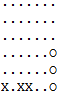
\includegraphics{Figures/gamestate}
   \end{center}
   \caption{Sample gamestate}
   \label{fig:gamestate}
\end{figure} 
When ranking offensively, lines of the player's counters are considered and when ranking defensively, lines of the opponent's counters. Looking at figure \ref{fig:gamestate} again, if it is player1's turn (represented by the X characters) then the highest ranked defensive move will be the move for column 7, since player2 (the O's) has three counters in that column.
\\Once each move is ranked, one of them is then selected and played. The selection is done according to various probabilities which make up the individual's genotype.

\subsection{Designing the Genotype}
Again, because of the time constraints caused by problems with adding The Arena functionality, the genotype of the individuals in the population was not as well developed as intended. The genotype chosen encoded the probabilities of selecting moves in a few simplistic situations. The author had hoped to try and encode some of the strategic rules defined by Victor Allis\cite{connect4} in the genotype but was not able to because of time limitations. 
\\The implemented genotype is made up of three chromosomes, the first two made up of four genes and the last made up of seven.

\subsubsection{Chromosome One}
The first chromosome encodes various probabilities for when the individual is player1.
\begin{itemize}
  \item{Gene 1: encodes the probability of playing a counter in the middle board position on the first move of the game. By playing in the middle position, it has been proven that player1 will always win the game if both players play perfectly from there on\cite{connect4}}
  \item{Gene 2: encodes the probability of finishing a three in a row for player1}
  \item{Gene 3: encodes the probability of blocking a three in a row for player2}
  \item{Gene 4: encodes the probability of choosing a offensive move from the ranked move set}
\end{itemize}
If it's the first move of the game, the probability in gene 1 is checked to see if player1 plays in the middle column, if not, then player1 plays a random move. Whenever there is a three in a row found, the corresponding probability is checked to see whether or not to block or finish it. Whenever no other move has been selected, the probability in gene 4 is checked, if it passes then an offensively ranked move is chosen, if not then a defensively ranked move is selected.

\subsubsection{Chromosome Two}
The second chromosome encodes various probabilities for when the individual is player1.
\begin{itemize}
  \item{Gene 1: encodes the probability of playing a counter in the middle board position on the first move of the game. This gene is never used, it is included only to make chromosome one and two the same length for easy coding}
  \item{Gene 2: encodes the probability of finishing a three in a row for player2}
  \item{Gene 3: encodes the probability of blocking a three in a row for player1}
  \item{Gene 3: encodes the probability of choosing a offensive move from the ranked move set}
\end{itemize}
Whenever there is a three in a row found, the corresponding probability is checked to see whether or not to block or finish it. Whenever no other move has been selected, the probability in gene 4 is checked, if it passes then an offensively ranked move is chosen, if not then a defensively ranked move is selected.

\subsubsection{Chromosome Three}
The final chromosome simply encodes the probability of selecting each move in the ranked move set. Because there is no constraint that the values of the genes in this chromosome must add up to exactly 1, the probabilities are scaled such that they add up to exactly 1 before they are used to select a move from the move set.

\subsection{Testing}
\label{sec:p2test}
Once developed, the algorithms were tested with a small number of individuals (2-4) for 1000 generations to ensure that the algorithms were working as intended and optimising. It also gave some performance by which the training process could be planned. The real testing would come after the algorithms had been trained.

\subsubsection{Training}
The training process was the most important stage of the development of the project. It involved letting the algorithms optimise in The Arena. When the gantt chart for the project was drawn up, it was unknown how long the training process would take, so a period of four weeks was allocated. Now, with the performance benchmarks of the initial tests, an estimate of the training time could be calculated. The initial testing has shown that 400 games took approximately 20 minutes to run. If 400 games was taken to be one generation, this gave a population of 20 individuals. This gave an approximate training time for 1000 generations of two weeks.
\\Due to unforeseen circumstances, training started approximately a week late, so a population size of 20 was chosen since this would still leave a weeks contingency. It was not possible to train the algorithms in one large tournament, due to memory limitations, so instead it was trained in small tournaments, each covering 5-10\% of the required games.
\\The execution of the first tournament with 20 individuals took longer than anticipated. The first tournament was of 20000 games, 5\% of the total number of games and it took over a day to finish. Extrapolating that execution time over the rest of the training process, It looked like the training process would overrun. As such, the population size was reduced to 10 individuals. This allowed the training process to finish on time, but may have limited the optimisation of the algorithms.

\subsubsection{Training Parameters}
As mentioned above, the population size was set to 10 individuals, the number of chromosomes to 3, with 4, 4 and 7 genes respectively. The remaining parameters were kept similar to those used in testing phase one (see section \ref{sec:p1test}). The selection and recombination modes used to compare the project to Shark implementations were chosen for phase 2 testing. The complete list of testing parameters will be listed in the next section.

\subsubsection{Testing Process}
After the training period was completed, the system could be be tested to see how effectively it had learnt to play Connect 4. This would be done in two ways, firstly each algorithm would play 50 games against the author; 25 as player1, 25 as player2, and secondly, each algorithm would play 1000 games against the recursive player module provided by The Arena; 500 as player1, 500 as player2. This module is known to play very well, especially when given a large turn limit. Various turn lengths would be used to limit the performance of the recursive player and to try and find a time limit where the algorithm matched the recursive player. For each algorithm, only the best individual was used when playing against the author and the recursive module.